\section{Phonetic Transcriptions}
\label{ch:phonetic}
IST has created time aligned phonetic transcriptions
for the Linguometer data. The transcriptions have been automatically
generated with \emph{forced alignment} based on the orthographic
transcriptions included in the database, a lexicon, and speaker
independent phonetic models for Italian. The phonetic models are
Gaussian mixure based hidden Markov models trained using the RefRec
scripts \cite{gs:LindbergEtAl2000} on the SpeechDat corpus (European
project, Contract LE2-4001). The corpus contains recordings of more than
three thousand speakers of different age, gender, and accent. The
SpeechDat lexicon was used to convert orthographic into phonetic
transcriptions. Out of vocabulary words were added to the lexicon,
including the pseudo-words used in the
database. Table~\ref{tab:linguometer:transcriptions:lexicon} lists the
words and their pronunciations specified in SAMPA symbols
(\url{http://www.phon.ucl.ac.uk/home/sampa/}). As a
reference, Table~\ref{tab:linguometer:transcriptions:sampa} contains
the complete set of SAMPA symbols for Italian.

\begin{table}
\scriptsize
\centering
\begin{tabular}{ll|ll|ll}\hline\hline
word & pronunciation & word & pronunciation & word & pronunciation \\ \hline
accento & \texttt{ a ttS E n t o} & ancora & \texttt{ a n k o r a} & ba & \texttt{ b a} \\
bacco & \texttt{ b a kk o} & baffo & \texttt{ b a ff o} & bi & \texttt{ b i} \\
biro & \texttt{ b i r o} & birra & \texttt{ b i rr a} & bronzo & \texttt{ b r o n dz o} \\
buchi & \texttt{ b u k i} & bufalo & \texttt{ b u f a l o} & buffo & \texttt{ b u ff o} \\
calza & \texttt{ k a l ts a} & carretto & \texttt{ k a rr e tt o} & carro & \texttt{ k a rr o} \\
cefalo & \texttt{ tS e f a l o} & ceffo & \texttt{ tS e ff o} & cero & \texttt{ tS E r o} \\
ci & \texttt{ tS i} & cirro & \texttt{ tS i rr o} & da & \texttt{ d a} \\
di & \texttt{ d i} & fa & \texttt{ f a} & faro & \texttt{ f a r o} \\
farro & \texttt{ f a rr o} & fascia & \texttt{ f a SS a} & fazzoletto & \texttt{ f a tts o l e tt o} \\
fi & \texttt{ f i} & fu & \texttt{ f u} & gelato & \texttt{ dZ e l a t o} \\
gelo & \texttt{ dZ e l o} & ghiro & \texttt{ g i r o} & gi & \texttt{ dZ i} \\
giallo & \texttt{ dZ a ll o} & gli & \texttt{ L i} & gnu & \texttt{ J u} \\
goffo & \texttt{ g o ff o} & gozzo & \texttt{ g O tts o} & gru & \texttt{ g r u} \\
gufo & \texttt{ g u f o} & la & \texttt{ l a} & lava & \texttt{ l a v a} \\
legno & \texttt{ l e JJ o} & li & \texttt{ l i} & ma & \texttt{ m a} \\
mamma & \texttt{ m a mm a} & matto & \texttt{ m a tt o} & mattone & \texttt{ m a tt o n e} \\
mi & \texttt{ m i} & mirra & \texttt{ m i rr a} & mito & \texttt{ m i t o} \\
moro & \texttt{ m o r o} & muffa & \texttt{ m u ff a} & na & \texttt{ n a} \\
ni & \texttt{ n i} & nome & \texttt{ n o m e} & notaio & \texttt{ n o t a j o} \\
papa & \texttt{ p a p a} & pappa & \texttt{ p a pp a} & pi & \texttt{ p i} \\
pozzo & \texttt{ p O tts o} & psicologo & \texttt{ p s i k o l o g o} & sa & \texttt{ s a} \\
sci & \texttt{ S i} & scia & \texttt{ S i a} & scoglio & \texttt{ s k O LL o} \\
semi & \texttt{ s E m i} & sera & \texttt{ s E r a} & serra & \texttt{ s E rr a} \\
si & \texttt{ s i} & strada & \texttt{ s t r a d a} & su & \texttt{ s u} \\
terra & \texttt{ t E rr a} & ti & \texttt{ t i} & toro & \texttt{ t o r o} \\
tu & \texttt{ t u} & tuffo & \texttt{ t u ff o} & tufo & \texttt{ t u f o} \\
uovo & \texttt{ w O v o} & va & \texttt{ v a} & vaso & \texttt{ v a z o} \\
vassoio & \texttt{ v a ss o j o} & vi & \texttt{ v i} & vu & \texttt{ v u} \\
yogurt & \texttt{ j o g u r t} & zi & \texttt{ ts i} &  & \\\hline\hline\end{tabular}

\caption{Pronunciation model for the Linguometer corpus (SAMPA symbols)}
\label{tab:linguometer:transcriptions:lexicon}
\end{table}

\begin{longtable}{|c|>{\sffamily}c|c|c|c|} \hline
IPA & SAMPA & Word & IPA & SAMPA \\ \hline
\hline \multicolumn{5}{|l|}{\textbf{6 single and 6 geminate plosives}} \\ \hline
\textipa{p} & \texttt{p} & pane & \textipa{pane} & \texttt{pane} \\ 
\textipa{b} & \texttt{b} & banco & \textipa{banko} & \texttt{banko} \\ 
\textipa{t} & \texttt{t} & tana & \textipa{tana} & \texttt{tana} \\ 
\textipa{d} & \texttt{d} & danno & \textipa{dan:o} & \texttt{danno} \\ 
\textipa{k} & \texttt{k} & cane & \textipa{kane} & \texttt{kane} \\ 
\textipa{g} & \texttt{g} & gamba & \textipa{gamba} & \texttt{gamba} \\ 
\textipa{p:} & \texttt{pp} & coppa & \textipa{kOp:a} & \texttt{kOppa} \\ 
\textipa{b:} & \texttt{bb} & gobba & \textipa{gOb:a} & \texttt{gObba} \\ 
\textipa{t:} & \texttt{tt} & zitto & \textipa{\texttslig it:o} & \texttt{tsitto} \\ 
\textipa{d:} & \texttt{dd} & cadde & \textipa{kad:e} & \texttt{kadde} \\ 
\textipa{k:} & \texttt{kk} & nocca & \textipa{nOk:a} & \texttt{nOkka} \\ 
\textipa{g:} & \texttt{gg} & fugga & \textipa{fug:a} & \texttt{fugga} \\ 
\hline \multicolumn{5}{|l|}{\textbf{4 single and 4 geminate affricates}} \\ \hline
\textipa{\texttslig} & \texttt{ts} & zitto & \textipa{\texttslig it:o} & \texttt{tsitto} \\ 
\textipa{\textdzlig} & \texttt{dz} & zona & \textipa{\textdzlig Ona} & \texttt{dzOna} \\ 
\textipa{\textteshlig} & \texttt{tS} & cena & \textipa{\textteshlig ena} & \texttt{tSena} \\ 
\textipa{\textdyoghlig} & \texttt{dZ} & gita & \textipa{\textdyoghlig ita} & \texttt{dZita} \\ 
\textipa{\texttslig:} & \texttt{tts} & bozza & \textipa{bO\texttslig:a} & \texttt{bOttsa} \\ 
\textipa{\textdzlig:} & \texttt{ddz} & mezzo & \textipa{mE\textdzlig:o} & \texttt{mEddzo} \\ 
\textipa{\textteshlig:} & \texttt{ttS} & braccio & \textipa{bra\textteshlig:o} & \texttt{brattSo} \\ 
\textipa{\textdyoghlig:} & \texttt{ddZ} & oggi & \textipa{O\textdyoghlig:i} & \texttt{OddZi} \\ 
\hline \multicolumn{5}{|l|}{\textbf{5 single and 4 geminate fricatives}} \\ \hline
\textipa{f} & \texttt{f} & fame & \textipa{fame} & \texttt{fame} \\ 
\textipa{v} & \texttt{v} & vano & \textipa{vano} & \texttt{vano} \\ 
\textipa{s} & \texttt{s} & sano & \textipa{sano} & \texttt{sano} \\ 
\textipa{z} & \texttt{z} & sbaglio & \textipa{zbaL:o} & \texttt{zbaLLo} \\ 
\textipa{S} & \texttt{S} & scendo & \textipa{Sendo} & \texttt{Sendo} \\ 
\textipa{f:} & \texttt{ff} & beffa & \textipa{bEf:a} & \texttt{bEffa} \\ 
\textipa{v:} & \texttt{vv} & bevvi & \textipa{bev:i} & \texttt{bevvi} \\ 
\textipa{s:} & \texttt{ss} & cassa & \textipa{kas:a} & \texttt{kassa} \\ 
\textipa{S:} & \texttt{SS} & ascia & \textipa{aS:a} & \texttt{aSSa} \\ 
\hline \multicolumn{5}{|l|}{\textbf{3 single and 3 geminate nasals}} \\ \hline
\textipa{m} & \texttt{m} & molla & \textipa{mOl:a} & \texttt{mOlla} \\ 
\textipa{n} & \texttt{n} & nocca & \textipa{nOk:a} & \texttt{nOkka} \\ 
\textipa{\ng} & \texttt{J} & gnocco & \textipa{NOk:o} & \texttt{JOkko} \\ 
\textipa{m:} & \texttt{mm} & grammo & \textipa{gram:o} & \texttt{grammo} \\ 
\textipa{n:} & \texttt{nn} & panna & \textipa{pan:a} & \texttt{panna} \\ 
\textipa{\ng:} & \texttt{JJ} & bagno & \textipa{baN:o} & \texttt{baJJo} \\ 
\hline \multicolumn{5}{|l|}{\textbf{3 single and 3 geminate liquids and 2 semivowels}} \\ \hline
\textipa{r} & \texttt{r} & rete & \textipa{rete} & \texttt{rete} \\ 
\textipa{l} & \texttt{l} & lama & \textipa{lama} & \texttt{lama} \\ 
\textipa{L} & \texttt{L} & gli & \textipa{Li} & \texttt{Li} \\ 
\textipa{r:} & \texttt{rr} & ferro & \textipa{fEr:o} & \texttt{fErro} \\ 
\textipa{l:} & \texttt{ll} & colla & \textipa{kOl:a} & \texttt{kOlla} \\ 
\textipa{L:} & \texttt{LL} & foglia & \textipa{fOL:a} & \texttt{fOLLa} \\ 
\textipa{J} & \texttt{j} & ieri & \textipa{Jeri} & \texttt{jeri} \\ 
\textipa{w} & \texttt{w} & uomo & \textipa{wOmo} & \texttt{wOmo} \\ 
\hline \multicolumn{5}{|l|}{\textbf{7 vowels}} \\ \hline
\textipa{i} & \texttt{i} & mite & \textipa{mite} & \texttt{mite} \\ 
\textipa{e} & \texttt{e} & rete & \textipa{rete} & \texttt{rete} \\ 
\textipa{E} & \texttt{E} & meta & \textipa{mEta} & \texttt{mEta} \\ 
\textipa{a} & \texttt{a} & rata & \textipa{rata} & \texttt{rata} \\ 
\textipa{O} & \texttt{O} & moto & \textipa{mOto} & \texttt{mOto} \\ 
\textipa{o} & \texttt{o} & dove & \textipa{dove} & \texttt{dove} \\ 
\textipa{u} & \texttt{u} & muto & \textipa{muto} & \texttt{muto} \\ 
\hline\caption{SAMPA symbols for Italian}
\label{tab:linguometer:transcriptions:sampa}
\end{longtable}


\subsection{Limitations}
There are a number of limitations when creating phonetic
transcriptions with the method described above. The main problems are:
\begin{itemize}
\item the lexicon specifies the canonical pronunciation for each
  word. Possible deviations from the canonical pronunciation are not
  captured by the method. A possible solution would be to specify a
  number of anternative pronunciations for each word and select
  automatically the one that best fits the data. However, this problem
  is of secondary impoprtance in this case, as the variation of
  pronunciation is limited when the subject reads a set of isolated
  words,
\item the time resolution of the method is 10 msec,
\item the acoustic models were trained on telephone speech recorded at
  8 kHz sampling fequency. Even though the Linguometer material was
  filtered and downsampled to match the training data, there
  might be a residual channel mismatch.
\end{itemize}


\subsection{Examples}

\begin{tabular}{l}
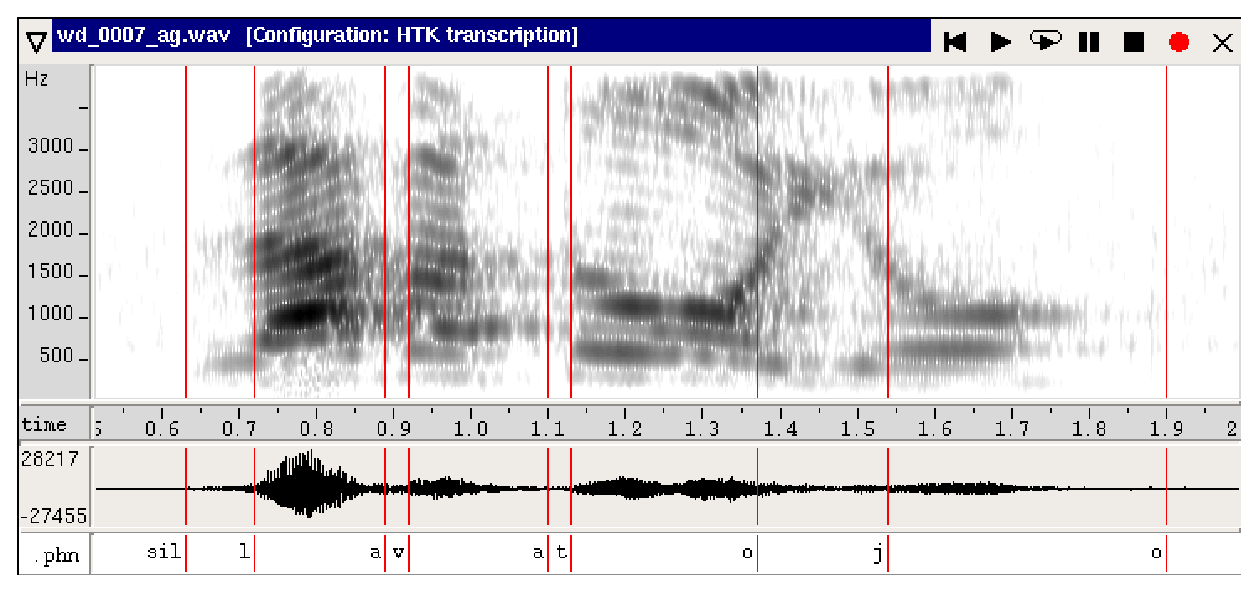
\epsfig{file=include/linguometer/images/exp_0001_seq_0000_wd_0007_lavatoio.eps,width=1.00\textwidth} \\
lavatoio \\
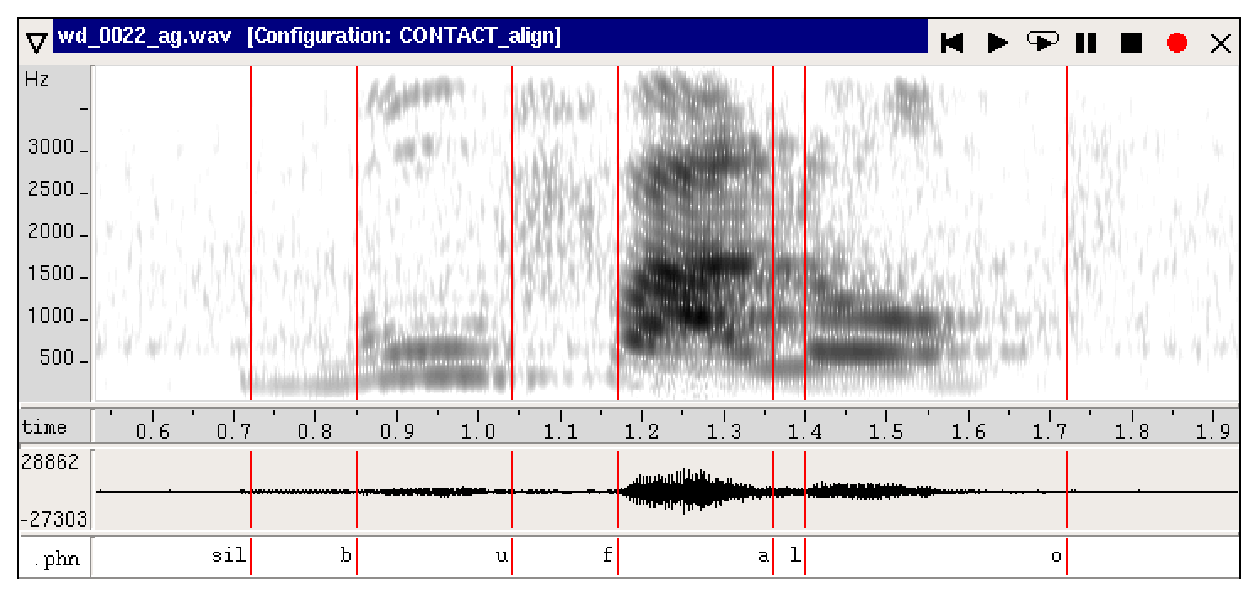
\epsfig{file=include/linguometer/images/exp_0001_seq_0000_wd_0022_bufalo.eps,width=1.00\textwidth} \\
bufalo \\
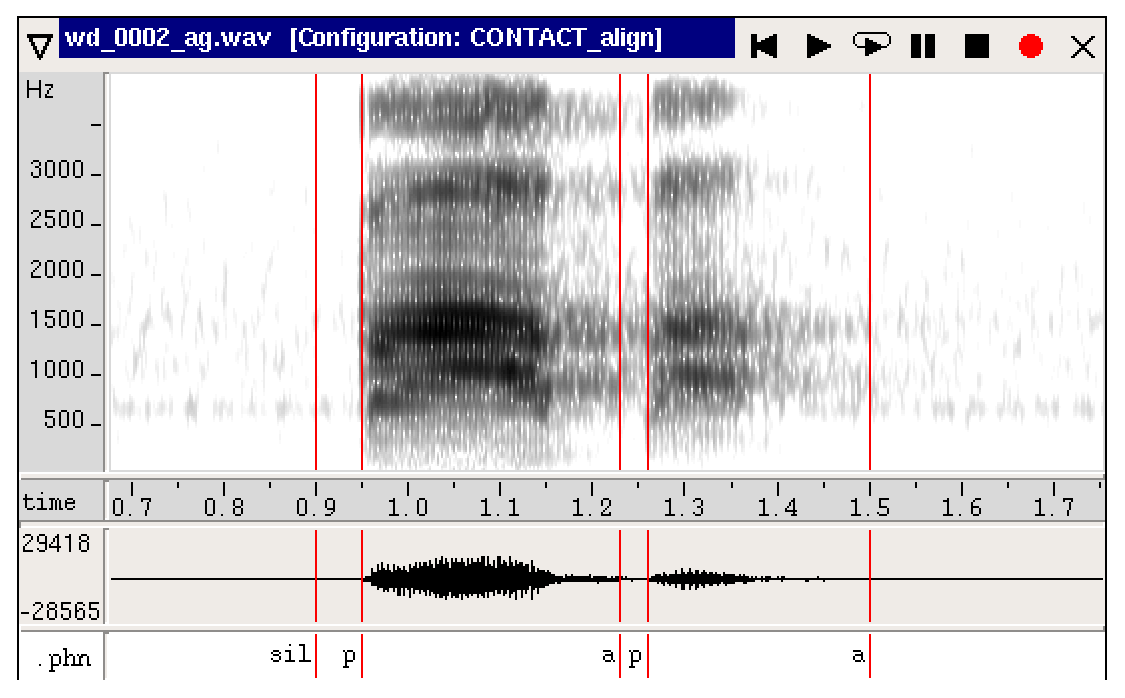
\epsfig{file=include/linguometer/images/exp_0005_seq_0000_wd_0002_papa.eps,width=0.60\textwidth} \\
papa
\end{tabular}

